% XeLaTeX can use any Mac OS X font. See the setromanfont command below.
% Input to XeLaTeX is full Unicode, so Unicode characters can be typed directly into the source.

% The next lines tell TeXShop to typeset with xelatex, and to open and save the source with Unicode encoding.

%!TEX TS-program = xelatex
%!TEX encoding = UTF-8 Unicode

\documentclass[14pt]{article}
%\usepackage[chordbk]{songbook} 
\usepackage{gchords}  
\usepackage{geometry}
\usepackage{rotating}
\usepackage{multicol}
\usepackage{enumitem,xcolor}
\usepackage{hyperref}
\hypersetup{
    colorlinks,
    citecolor=black,
    filecolor=black,
    linkcolor=black,
    urlcolor=black
}

\geometry{a4paper}                 
\usepackage{graphicx}
\usepackage{amssymb}

% Will Robertson's fontspec.sty can be used to simplify font choices.
% To experiment, open /Applications/Font Book to examine the fonts provided on Mac OS X,
% and change "Hoefler Text" to any of these choices.

\usepackage{fontspec,xltxtra,xunicode}

\defaultfontfeatures{Mapping=tex-text}
%\setromanfont[Mapping=tex-text]{Hoefler Text}
%\setsansfont[Scale=MatchLowercase,Mapping=tex-text]{Gill Sans}
%\setmonofont[Scale=MatchLowercase]{Andale Mono}
\title{Different Class}
\author{Songbook}
\date{}                                           % Activate to display a given date or no date


\font\fingerfont=cmr3

%Override LaTEX defaults

\newcommand{\up}[1]{\textsuperscript{#1}}
\renewcommand\thesection{} % No number in section title


% Chords 

\let\oldchord\chord
\renewcommand{\chord}[3]{\oldchord{#1}{#2}{\sffamily#3}}
\newcommand{\atfret}[2]{

	\parbox[c][3.25em][b]{7pt}{

			\makebox[10pt]{#1}
			\makebox[10pt]{\git{\small(#2th fret)}}
			%\raisebox{-2.5ex}{\git{(#2th fret)}}
		}
}

% Chords with dots (without fingers' numbers)
%%A
%
%\newcommand{\AMaj}{\chord{t}{x, o, p2, p2, p2, o}{A}}
%
%
%%B
%\newcommand{\BMaj}{\chord{t}{x, p2, p1, p4, o, p2}{B}}
%\newcommand{\BFlat}{\chord{t}{x, p1, o, p3, p3, p1}{Bb}}
%\newcommand{\BMajsusFour}{\chord{t}{x, p2, p4, p4, o, o}{B\up{sus4}}}
%
%% C
%\newcommand{\CMaj}{\chord{t}{x, p3, p2, o, p1, o}{C}}
%\newcommand{\CMajSeven}{\chord{t}{x, p3, p2, o, o, o}{C\up{maj7}}}
%\newcommand{\CSeven}{\chord{t}{x, p3, p2, p3, p1, o}{C\up7}}
%\newcommand{\CMajShE}{\chord{8}{p1, p3, p3, p2, p1, p1}{\atfret{C}{8}}}
%\newcommand{\CMajsusFour}{\chord{t}{x, p3, p3, o, p1, o}{C\up{sus4}}}
%\newcommand{\Cm}{\chord{t}{x, p3, p1, o, p1, p3}{Cm}}
%
%
%
%% D
%
%\newcommand{\DMaj}{\chord{t}{x, x, o, p2, p3, p2}{D}}
%\newcommand{\DSeven}{\chord{t}{x, x, o, p2, p1, p2}{D\up7}}
%\newcommand{\DMajShA}{\chord{5}{x, p1, p3, p3, p3, p1}{\atfret{D}{5}}}
%\newcommand{\Dm}{\chord{t}{x, x, o, p2, p3, p1}{Dm}}
%
%% E
%
%\newcommand{\EMaj}{\chord{t}{o, p2, p2, p1, o, o}{E}}
%\newcommand{\Em}{\chord{t}{o, p2, p2, o, o, o}{Em}}
%\newcommand{\EmShAm}{\chord{7}{x, p1, p3, p3, p2, p1}{\atfret{Em}{7}}}
%
%\newcommand{\EmaddC}{\chord{t}{o, p2, p2, o, p1, o}{Em\up{addC}}}
%\newcommand{\EmSix}{\chord{t}{o, p2, p2, o, p2, o}{Em\up{6}}}
%
%
%% F
%
%\newcommand{\FMaj}{\chord{t}{n, p3, p3, p2, n, n}{FakeF}}
%\newcommand{\FMajsusFour}{\chord{t}{n, n, p3, p3, n, n}{FakeF\up{sus4}}}
%
%
%% F#
%
%\newcommand{\Fshm}{\chord{t}{p2, p4, p4, p2, p2, p2}{F\#m}}
%
%
%%G
%\newcommand{\GMaj}{\chord{t}{p3, p2, o,o, o, p3}{G}}
%\newcommand{\GMajSeven}{\chord{t}{p3, p2, o,o, o, p2}{G\up{maj7}}}
%\newcommand{\GSeven}{\chord{t}{p3, p2, o,o, o, p1}{G\up 7}}
%\newcommand{\GMajShE}{\chord{3}{p1, p3, p3,p2, p1, p1}{\atfret{G}{3}}}
%\newcommand{\Gm}{\chord{t}{p4, p1, o, o, p4, p4}{Gm}}

%A

\newcommand{\AMaj}{\chord{t}{x, o, p2, p2, p2, o}{A}}


%B
\newcommand{\BMaj}{\chord{t}{x, f2p2, f1p1, f4p4, o, f3p2}{B}}
\newcommand{\BFlat}{\chord{t}{x, f1p1, o, f3p3, f4p3, f2p1}{Bb}}
\newcommand{\BMajsusFour}{\chord{t}{x, f1p2, f3p4, f4p4, o, o}{B\up{sus4}}}

% C
\newcommand{\CMaj}{\chord{t}{x, p3, p2, o, p1, o}{C}}
\newcommand{\CMajSeven}{\chord{t}{x, p3, p2, o, o, o}{C\up{maj7}}}
\newcommand{\CSeven}{\chord{t}{x, p3, p2, p3, p1, o}{C\up7}}
\newcommand{\CMajShE}{\chord{8}{p1, p3, p3, p2, p1, p1}{\atfret{C}{8}}}
\newcommand{\CMajsusFour}{\chord{t}{x, p3, p3, o, p1, o}{C\up{sus4}}}
\newcommand{\Cm}{\chord{t}{x, f3p3, f1p1, o, f2p1, f4p3}{Cm}}



% D

\newcommand{\DMaj}{\chord{t}{x, x, o, p2, p3, p2}{D}}
\newcommand{\DSeven}{\chord{t}{x, x, o, p2, p1, p2}{D\up7}}
\newcommand{\DMajShA}{\chord{5}{x, p1, p3, p3, p3, p1}{\atfret{D}{5}}}
\newcommand{\Dm}{\chord{t}{x, x, o, f2p2, f3p3, f1p1}{Dm}}

% E

\newcommand{\EMaj}{\chord{t}{o, p2, p2, p1, o, o}{E}}
\newcommand{\Em}{\chord{t}{o, p2, p2, o, o, o}{Em}}
\newcommand{\EmShAm}{\chord{7}{x, p1, p3, p3, p2, p1}{\atfret{Em}{7}}}

\newcommand{\EmaddC}{\chord{t}{o, p2, p2, o, p1, o}{Em\up{addC}}}
\newcommand{\EmSix}{\chord{t}{o, p2, p2, o, p2, o}{Em\up{6}}}


% F

\newcommand{\FMaj}{\chord{t}{n, f3p3, f4p3, f2p2, n, n}{FakeF}}
\newcommand{\FMajsusFour}{\chord{t}{n, n, f3p3, f4p3, n, n}{FakeF\up{sus4}}}


% F#

\newcommand{\Fshm}{\chord{t}{p2, p4, p4, p2, p2, p2}{F\#m}}


%G
\newcommand{\GMaj}{\chord{t}{p3, p2, o,o, o, p3}{G}}
\newcommand{\GMajSeven}{\chord{t}{p3, p2, o,o, o, p2}{G\up{maj7}}}
\newcommand{\GSeven}{\chord{t}{p3, p2, o,o, o, p1}{G\up 7}}
\newcommand{\GMajShE}{\chord{3}{p1, p3, p3,p2, p1, p1}{\atfret{G}{3}}}
\newcommand{\Gm}{\chord{t}{f4p4, f1p1, o, o, p4, p4}{Gm}}



\newcommand{\git}[1]{\color{gray}{\textit{#1}}\color{black}}


\newenvironment{myenumerate}{%
  \edef\backupindent{\the\parindent}
  \begin{enumerate}[label=\color{gray}\theenumi]
  \setlength{\parindent}{\backupindent}
}{\end{enumerate}}

\setlength{\parindent}{0cm}

\newenvironment{song}[2]
{
	\begin{center}
		\section{#1}
		#2
	\end{center}
	\begin{multicols}{2}
		\normalsize
		\begin{myenumerate}
}{
		\end{myenumerate}
	\end{multicols}
	\newpage
}


\definecolor{blue}{rgb}{0.2, 0.5, 0.5}
\newenvironment{SongVerse}
{
	\item
}{
\vspace{10pt}
}
\newcommand{\ch}[1]{
	\makebox[0pt][l]{\raisebox{2.5ex}{\color{blue}\sffamily \,\,#1}}
}


% \def\numfrets{4}

\begin{document}

\maketitle

\newpage

\tableofcontents 
\newpage

\begin{song}{Mis-Shapes}{

    \git{Verse}

	\mbox{ \AMaj \EMaj \Fshm \DMaj \DSeven}

    \git{Chorus}

	\mbox{ \GMaj \GMajSeven \GSeven \CMaj \CMajSeven \CSeven }
	

	\mbox{ \Em \EmSix \EmaddC }

}

	 \begin{SongVerse}
		\ch{A}{Mis-shapes}, mistakes, misfits. 

		\ch{E}{Raised} on a diet of broken biscuits, oh \ch{F\#m}{}

		We don't look the same as you \ch{D}{}
		
		We don't do the things you do,
		
		But \ch{D7}{we} live around here too, oh really. 
	 \end{SongVerse}

	 \begin{SongVerse}
		\ch{A}{Mis-shapes}, mistakes, misfits,

		We'd \ch{E}{like} to go to town but we can't risk it, oh \ch{F\#m}{} 

		'Cos they just want to keep us out. \ch{D}{} 
		
		You could end up with a smack in the mouth

		\ch{D7}{Just} for standing out, now really.
	 \end{SongVerse}

	 \begin{SongVerse}

		\ch{A}Brothers, sisters, can't you \ch{E}see? 

		The future's owned by you and \ch{F\#m}me. 

		There won't be fighting in the \ch{D}street. 

		They think they've got us beat, 

		But \ch{D\up7}revenge is going to be so sweet. 
	\end{SongVerse}

	\begin{SongVerse}
		
		\ch{G} \quad We're making a \ch{G\up{maj7}}move, 

		we're making it \ch{G\up 7}now. 

		We're coming out of the sidelines. 

		\ch{C}\quad Just put your \ch{C\up{maj7}}hands up -- it's a \ch{C\up7}raid \ch{C}... \ch{C\up7}yeah.

		We want your \ch{Em}homes,

		we want your \ch{Em\up{addC}}lives,

		we want the \ch{Em6}things you won't \ch{Em\up{addC}}allow us. 

		We won't use \ch{Em}guns, 

		we won't use \ch{Em\up{addC}}bombs

		We'll use the \ch{Em6}one thing we've got \ch{Em\up{addC}}more of --

		that's our \ch{Em}minds. \ch{Em\up{addC}} \hspace{20pt} \ch{Em6} \qquad \ch{Em}

	\end{SongVerse}

	\begin{SongVerse}

		\ch{A} Check your lucky numbers.

		\ch{E}That much money could drag you under, oh. \ch{F\#m}

		What's the point of being rich \ch{D}

		if you can't think what to do 
		
		with it 

		'cos \ch{D\up7}you're so bleeding thick?

	\end{SongVerse}

	\begin{SongVerse}

		
		\ch{A} \quad Oh, we weren't supposed to \ch{E}be -- 

		we learnt too much at school now 

		\ch{F\#m} we can't help but see 

		that the \ch{D}future that you've got mapped out 

		is \ch{D\up7} nothing much to shout about. 

	\end{SongVerse}

	\begin{SongVerse}

		
		\ch{G} \quad We're making a \ch{G\up{maj7}}move, 

		we're making it \ch{G\up 7}now. 

		We're coming out of the sidelines. 

		\ch{C}\quad Just put your \ch{C\up{maj7}}hands up -- it's a \ch{C\up7}raid \ch{C}... \ch{C\up7}yeah.

		We want your \ch{Em}homes,

		we want your \ch{Em\up{addC}}lives,

		we want the \ch{Em6}things you won't \ch{Em\up{addC}}allow us. 

		We won't use \ch{Em}guns, 

		we won't use \ch{Em\up{addC}}bombs

		We'll use the \ch{Em6}one thing we've got \ch{Em\up{addC}}more of --

		that's our \ch{Em}minds. \ch{Em\up{addC}} \hspace{30pt} \ch{Em6} \qquad \ch{Em}

	\end{SongVerse}

	\begin{SongVerse}
				\ch{A}Brothers, sisters, can't you \ch{E}see? 

		The future's owned by you and \ch{F\#m}me. 

		There won't be fighting in the \ch{D}street. 

		They think they've got us beat, 

		But \ch{D\up7}revenge is going to be so sweet. 
	\end{SongVerse}

	\begin{SongVerse}		

		
		\ch{G} \quad We're making a \ch{G\up{maj7}}move, 

		we're making it \ch{G\up 7}now. 

		We're coming out of the sidelines. 

		\ch{C}\quad Just put your \ch{C\up{maj7}}hands up -- it's a \ch{C\up7}raid \ch{C}... \ch{C\up7}yeah.

		We want your \ch{Em}homes,

		we want your \ch{Em\up{addC}}lives,

		we want the \ch{Em6}things you won't \ch{Em\up{addC}}allow us. 

		We won't use \ch{Em}guns, 

		we won't use \ch{Em\up{addC}}bombs

		We'll use the \ch{Em6}one thing we've got \ch{Em\up{addC}}more of --

		that's our \ch{Em}minds. \ch{Em\up{addC}} \hspace{30pt} \ch{Em6} \qquad \ch{Em}

	 \end{SongVerse}

\end{song}
\begin{song}{Pencil Skirt}{
	
	\chordset[Verse]{ \CMaj \AMaj \DMaj \GMaj }
	\chordset[Chorus]{ \EmShAm \CMajShE \DMajShA \GMajShE}
	\vspace{1em}
	\tabset[Riff 1]{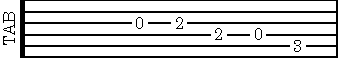
\includegraphics{tab/pencilskirt1}}%
	\tabset[Riff 2]{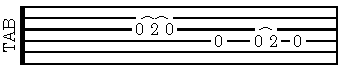
\includegraphics{tab/pencilskirt2}}
}


\begin{songverse}


\ch{Riff 1}\hspace{30pt}\ch{C}When you raise your pencil \ch{A}skirt like a 

\ch{D}veil before my \ch{G}eyes \ch{Riff 2}

 \ch{C}Like the look upon his \ch{A}face as he's

 
 \ch{D}zipping up his \ch{G}flies, \ch{Riff 2}oh


 \ch{C}But I \ch{A}know that


 \ch{D}you're engaged to \ch{G}him  \ch{Riff 2}, oh


\ch{C}\hspace{10pt}But I  \ch{A}know you \ch{D}want something 


to \ch{G}play with, baby

\end{songverse}

\begin{songchorus}

 \ch{Em}I'll be around when he's not in 
 
 town, oh \ch{C}


 Yeah I'll show you how you're 
 
 doing it wrong, oh \ch{Em}


 I really love it when you tell me 
 
 to stop, oh oh \ch{D}
                
 
 Oh it's turning me \ch{G}on

\end{songchorus}

\begin{songverse}

\ch{Riff 2}\hspace{30pt}\ch{C} Now you can tell some \ch{A}lies about the\ch{D}good times that you've \ch{G}had \ch{Riff 2}


\ch{C}But I've kissed your mother \ch{A}twice and


I'm work\ch{D}ing on your \ch{G}dad, oh baby


\end{songverse}

\begin{songchorus}

 \ch{Em}I'll be around when he's not in 
 
 town, oh \ch{C}


 Yeah I'll show you how you're 
 
 doing it wrong, oh \ch{Em}


 I really love it when you tell me 
 
 to stop, oh oh \ch{D}
                
 
 Oh it's turning me \ch{G}on

\end{songchorus}


\begin{songverse}
\ch{Riff 2}\hspace{30pt} \ch{C}If you look under the \ch{A}bed then I can \ch{D}see my house 

from \ch{G}here \ch{Riff 2}

 \ch{C}So just lie against  the \ch{A}wall and watch my  \ch{D}conscience disap\ch{G}pear, now baby oh


 \ch{Em}Yeah, I'll be around when he's not in town, oh
 
 
 \ch{C}Oh yeah, I'll show you how you're doing it wrong, oh
 
 
 \ch{Em}I really love it when you tell me to stop, oh oh
 
                  
 \ch{D}Oh it's turning me \ch{G}on, on, on, yeah

\end{songverse}


 \begin{songverse}[Bridge]

 \ch{Em}\hspace{10pt}I only come here cause I know it makes you sad
 
 
 
 \ch{C}\hspace{10pt}I only do it cause I know you know it's bad.
 
 
 
 Oh don't you \ch{Em}know it's ugly and it shouldn't be like that.
 
                          
 \ch{D}\hspace{10pt}Oh but oh it's turning me \ch{G}on, on, on, on, on, on, on.


\ch{C}  \hspace{15pt}  \ch{A} \hspace{15pt}   \ch{D}  \hspace{15pt}   \ch{G}
 \end{songverse}

\end{song}
\begin{song}{Common People}{
	
	\chordset[Intro]{ \CMaj \CMajsusFour }
	\chordset[Verse, Chorus]{ \CMaj \GMaj \FMaj }
	
}
	 \begin{songverse}
		\ch{A}{Mis-shapes}, mistakes, misfits. 

		\ch{E}{Raised} on a diet of broken biscuits, oh \ch{F\#m}{}

		We don't look the same as you \ch{D}{}
		
		We don't do the things you do,
		
		But \ch{D7}{we} live around here too, oh really. 
	 \end{songverse}

\end{song}
\begin{song}{Disco 2000}{
	
	\chordset[Intro]{ \FMaj \FMajsusFour \BMaj \BMajsusFour }	
	
	\chordset[Verse]{ \FMaj \BFlat }

	\chordset[Chorus]{ \Cm \BFlat \Dm \Gm \FMaj }
	
}
	\begin{songverse}
	
	Intro: F \quad  F\up{sus4} \quad B \quad B\up{sus4}
	\end{songverse}
	
	 \begin{songverse}	       
	 
		Well we were \ch{F}{born} within an hour of each other

		Our mothers said we could be sister and brother
              
		Your name is \ch{Bb}{Deborah}.  Deborah, it never suited you
         
		And they \ch{F}{said} that when we grew up 

		We'd get married and never split up
           
		We never \ch{Bb}{did}, although I often thought of it		 
	 \end{songverse}

	 \begin{songverse}	     
	                  
		Oh Deborah, do you \ch{Cm}{recall}?

		Your house was very small

		With wood chip on the wall
                         
		And when I came round to \ch{Cm}{call}

		You didn't notice me at all 		
	 \end{songverse}

	 \begin{songverse}
                          
		And I said, \ch{Bb}{lets} all meet up in the year 2000
                                        
		\ch{Dm}{Won't} it be strange when we're all fully \ch{Gm}{grown}
                                          
		Be there 2 o'clock by the \ch{Cm}{fountain} down the \ch{F}{road}

		\ch{Bb}{I} never knew that you'd get married 
                             
		\ch{Dm}{I} would be living down here on my \ch{Gm}{own}   

		On that damp and lonely \ch{Cm}{thursday} years \ch{F}{ago} 
	\end{songverse}

	\begin{songverse}
		
		You were the first girl at school to get breasts.
		
		Martyn said that yours were the best.
		
		The boys all loved you but I was a mess.
		
		I had to watch them trying to get you undressed.
		
		We were friends but that was as far as it went.
		
		I used to walk you home sometimes but it meant,
		oh it meant nothing to you,
		cos you were so popular.
	\end{songverse}
	
	 \begin{songverse}	     
	                  
		Oh Deborah, do you \ch{Cm}{recall}?

		Your house was very small

		With wood chip on the wall
                         
		And when I came round to \ch{Cm}{call}

		You didn't notice me at all 		
	 \end{songverse}

 \begin{songverse}
                          
		And I said, \ch{Bb}{lets} all meet up in the year 2000
                                        
		\ch{Dm}{Won't} it be strange when we're all fully \ch{Gm}{grown}
                                          
		Be there 2 o'clock by the \ch{Cm}{fountain} down the \ch{F}{road}

		\ch{Bb}{I} never knew that you'd get married 
                             
		\ch{Dm}{I} would be living down here on my \ch{Gm}{own}   

		On that damp and lonely \ch{Cm}{thursday} years \ch{F}{ago} 
	\end{songverse}

		Oh yeah,
		oh yeah.
	
	 \begin{songverse}	     
	                  
		Ah do you \ch{Cm}{recall}?

		Your house was very small

		With wood chip on the wall
                         
		And when I came round to \ch{Cm}{call}

		You didn't notice me at all 		
	 \end{songverse}

	\begin{songverse}
	
		And I said, \ch{Bb}{lets} all meet up in the year 2000
                                        
		\ch{Dm}{Won't} it be strange when we're all fully \ch{Gm}{grown}
                                          
		Be there 2 o'clock by the \ch{Cm}{fountain} down the \ch{F}{road}

		\ch{Bb}{I} never knew that you'd get married 
                             
		\ch{Dm}{I} would be living down here on my \ch{Gm}{own}   

		On that damp and lonely \ch{Cm}{thursday} years \ch{F}{ago} 
		
		Oh what are you doing Sunday baby.
		
		Would you like to come and meet me maybe?
		
		You can even bring your baby.
		
		Ohhh ooh ooh. Ooh ooh ooh ooh.
		
		What are you doing Sunday baby.
		
		Would you like to come and meet me maby?
		
		You can even bring your baby.
		
		Ooh ooh oh. Ooh ooh ooh ooh. Ooh ooh ooh ooh. Oh. 
	 \end{songverse}

\end{song}

\end{document}